\begin{boiboiboite}
	\propeau
	\propair
	\isentropiques
\end{boiboiboite}


\subsubsection{Efficacité d’un moteur}
\label{exo_efficacite_moteur}

	Le moteur Diesel d’une excavatrice a une efficacité de~\SI{40}{\percent} et développe une puissance continue de~\SI{80}{ch} (c’est-à-dire \SI{60}{\kilo\watt}). Il est alimenté par du carburant de capacité calorifique \SI{35}{\mega\joule\per\kilogram}.
	
	\begin{enumerate}
		\item Quelle est la consommation horaire de carburant de la machine ?
		\item Quelle est la puissance qu’elle rejette sous forme de chaleur dans le conduit d’échappement ?
	\end{enumerate}

\subsubsection{Efficacité d’un réfrigérateur}
\label{exo_efficacite_refrigerateur}

	Un réfrigérateur dont le \textsc{cop} est de~\num{1,2} doit extraire \SI{100}{\kilo\joule} d’un aliment placé dans la chambre froide. Combien d’énergie électrique doit-il consommer pour cela ? Quelle quantité de chaleur aura-t-il rejetée à la fin du refroidissement ?
	

\subsubsection{Efficacité d’une pompe à chaleur}
\label{exo_efficacite_thermopompe}

	Une pompe à chaleur dont le \textsc{cop} est de~\num{3,1} fournit une puissance de~\SI{4000}{\watt} à une habitation. Quelle est la puissance électrique consommée ? Quelle est la puissance absorbée à l’atmosphère ?


\subsubsection{Thermodynamique de soirée}
\label{exo_bieres}

	Un groupe d’étudiants assoiffés par un cours de thermodynamique interminable prépare le week-end en plaçant au réfrigérateur dix packs de six bouteilles contenant une boisson à base d’eau minérale (\cref{fig_six_pack}).
	
	Une expérience effectuée sur une bouteille montre qu’elle est constituée de~\SI{172}{\gram} de verre de capacité calorifique massique \SI{0,75}{\kilo\joule\per\kilogram\per\kelvin}, et qu’elle contient \SI{25}{\centi\liter} de liquide de capacité \SI{4,2}{\kilo\joule\per\kilogram\per\kelvin}.
	
	Lorsqu’ils sont placés au réfrigérateur, les packs sont à température ambiante (\SI{19}{\degreeCelsius}). Quatre heures plus tard, ils ont atteint la température de~\SI{5}{\degreeCelsius}.
	
	\begin{figure}[htp] %handmade
		\begin{center}
		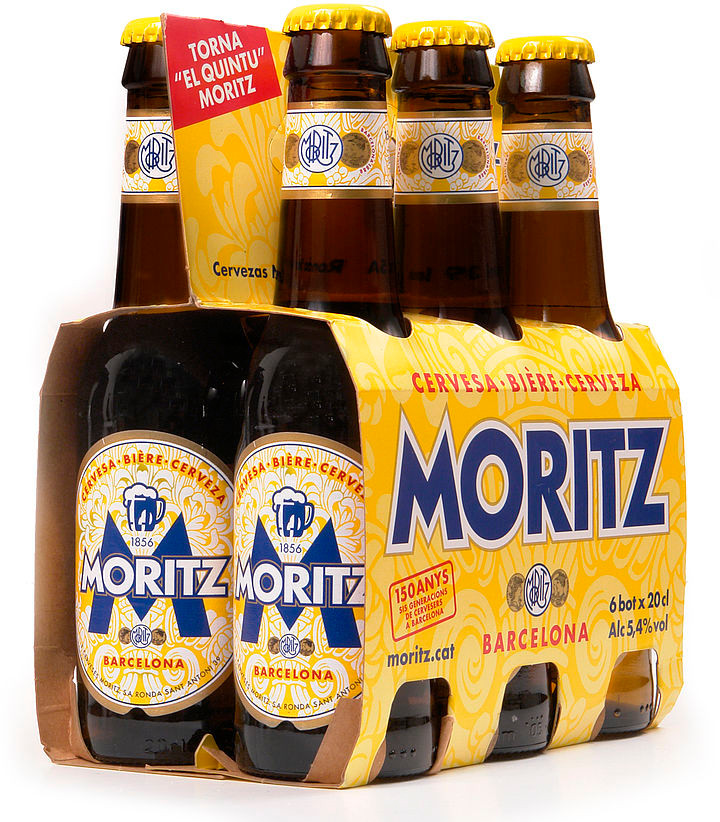
\includegraphics[width=2.5cm]{images/6-pack.jpg}
		\end{center}
		\supercaption{Pack de six bouteilles d’un liquide utilisé pour noyer l’exaspération propre à l’étude de la thermodynamique.}{\wcfile{El_"quintu"_de_Moritz.jpg}{photo} \ccby Moritz Barcelona}
		\label{fig_six_pack}
	\end{figure}
	
	Le réfrigérateur a un rendement de~\SI{95}{\percent}. Les parois du réfrigérateur, imparfaitement isolées, absorbent de la chaleur de la pièce avec une puissance de~\SI{10}{\watt}.

	
	\begin{enumerate}
		\item Quelle quantité d’énergie électrique le réfrigérateur a-t-il consommée pendant ces quatre heures ?
	\end{enumerate}
	
	L’opérateur du réseau électrique local applique un tarif de~\SI[per-mode=symbol]{0,15}{\euroo\per\kilo\watt\per\hour}.
	
	\begin{enumerate}
		\shift{1}
		\item Quel est le coût financier du refroidissement effectué ?
		\item La pièce dans laquelle le réfrigérateur est entreposé s’est-t-elle refroidie ou réchauffée ?
		\item La pièce se refroidira-t-elle si la porte du réfrigérateur est laissée ouverte ?
	\end{enumerate}


\subsubsection{Fonctionnement d’une pompe à chaleur}
\label{exo_fonctionnement_thermopompe}

	Décrivez le cycle thermodynamique suivi par le fluide à l’intérieur d’une pompe à chaleur, en indiquant le sens des flux de chaleur et l’emplacement (intérieur/extérieur) des différents composants.
	
	Pourquoi laisse-t-on le fluide se détendre dans une soupape, au lieu d’utiliser une turbine qui pourrait fournir du travail ?
	
	\textit{On peut aussi s’exercer en s’intéressant aux cycles et configurations d’un climatiseur, d’un réfrigérateur ou d’un moteur : quelle partie est réchauffée et à quelle température ?}


\subsubsection{Algèbre}
\label{exo_algebre_rendement_climatiseur}

	Montrez, à partir de la définition du rendement du climatiseur, que celui-ci peut s’exprimer selon la relation :
			\begin{equation}
				\eta_\text{climatiseur} = \frac{1}{\left| \frac{\dot Q_\out}{\dot Q_\inn} \right| - 1} \tag{\ref{rendement_réfrigérateur_qin_qout}}
			\end{equation}
	
	\textit{Cette démonstration nous sera utile au chapitre prochain (\S\ref{ch_efficacite_maximale_machines}). On peut aussi s’exercer en s’attaquant de la même manière aux équations~\ref{eq_rendement_moteur_qin_qout} et~\ref{eq_rendement_thermopompe_qin_qout}. Attention aux valeurs absolues !}
	
	
\subsubsection{Refroidissement d’une soufflerie}
\label{exo_refrigeration_soufflerie}

	La soufflerie cryogénique \textsc{etw} (pour \textit{European Transonic Windtunnel}, \cref{fig_souffleries}) permet la circulation d’azote dans un circuit fermé pour observer les écoulements autour de maquettes. Elle permet d’atteindre Mach~\num{0,8} à~\SI{4}{\bar} et~\SI{-200}{\celsius}, à l’aide d’une soufflante de~\SI{50}{\mega\watt}.
	
	Les parois de la soufflerie sont fortement isolées, de sorte que ses transferts thermiques avec l’extérieur sont négligeables comparés aux autres transferts énergétiques. Le système de refroidissement de l’azote a un \textsc{cop} de~\num{0,8}. 
	
	Lorsque la soufflerie fonctionne à plein régime, quelle puissance mécanique est consommée par le système de refroidissement ? Quelle puissance est rejetée sous forme de chaleur dans l’atmosphère ?

	\begin{figure}[htp]
		\begin{center}
			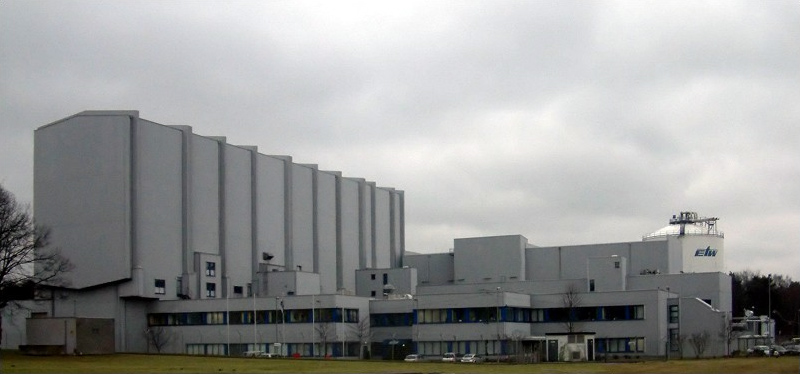
\includegraphics[width=0.8\columnwidth]{images/etw.jpg}
			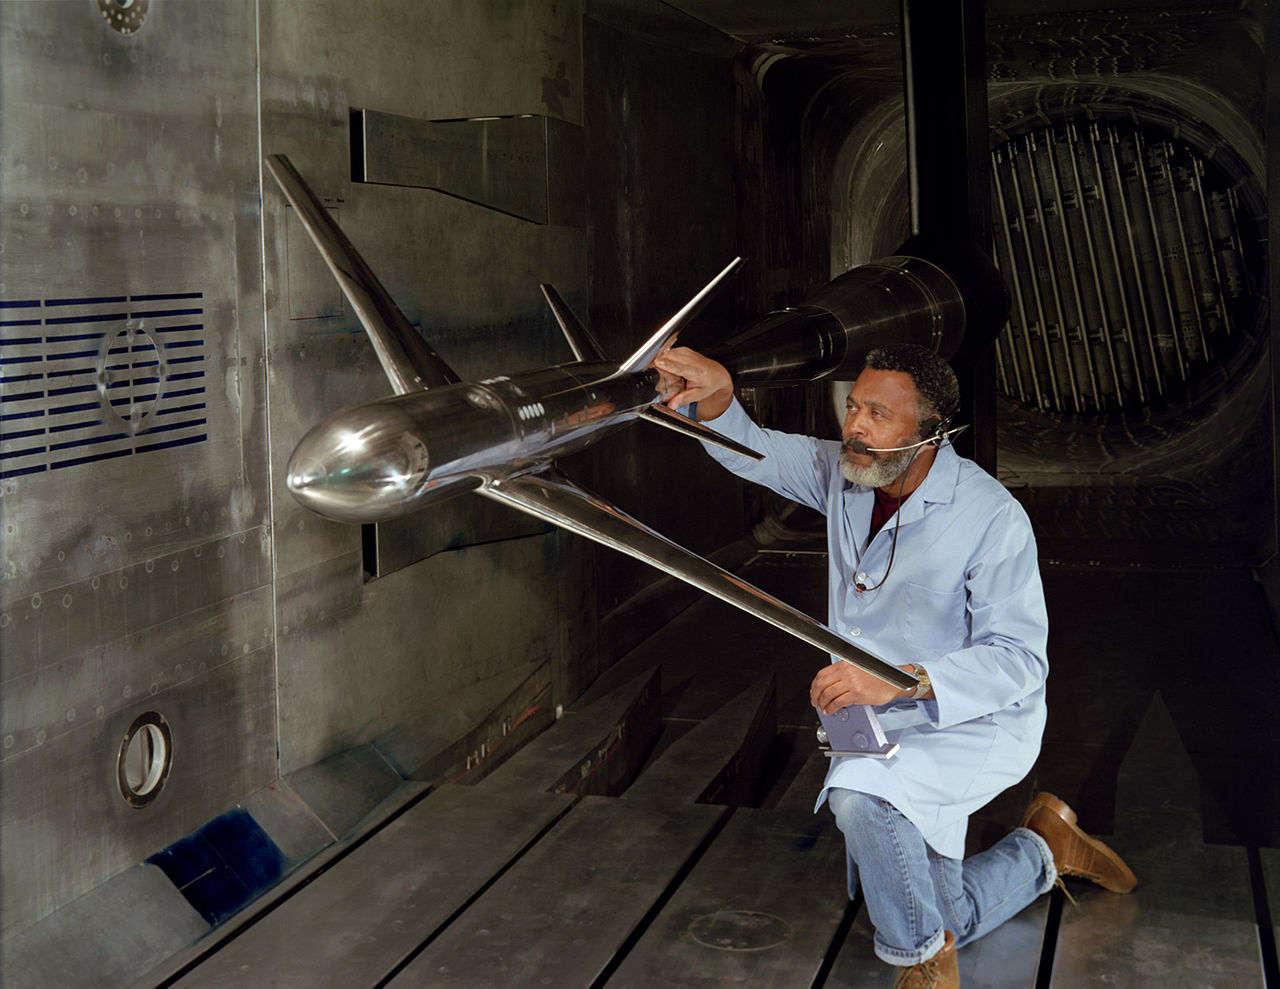
\includegraphics[width=0.8\columnwidth]{images/langley_transonic.jpg}
		\end{center}
		\supercaption{Bâtiments de l’\textsc{etw} (\textit{European Transonic Windtunnel}) à Köln et veine d’essais de la \textit{National Transonic Facility} de la \textsc{nasa}, de taille et capacités similaires.}{\wcfile{Etwrp.jpg}{Photo 1} \ccbysa par \wcu{Dantor}\\
		\wcfile{Pathfinder_I_with_Pressure_Wing_-_GPN-2000-001291.jpg}{Photo 2} \pd Fred Jones (\textsc{nasa})}
		\label{fig_souffleries}
	\end{figure}

\subsubsection{Génératrice d’électricité à turbine}
\label{exo_generatrice_electricite_turbine}

	Un turbomoteur est mis en place pour faire fonctionner une génératrice de courant électrique (\cref{fig_exo_turbomoteur}) ; il fonctionne avec un débit de~\SI{0,5}{\kilogram\per\second} d’air atmosphérique.
	
	\begin{figure}
		\begin{center}
		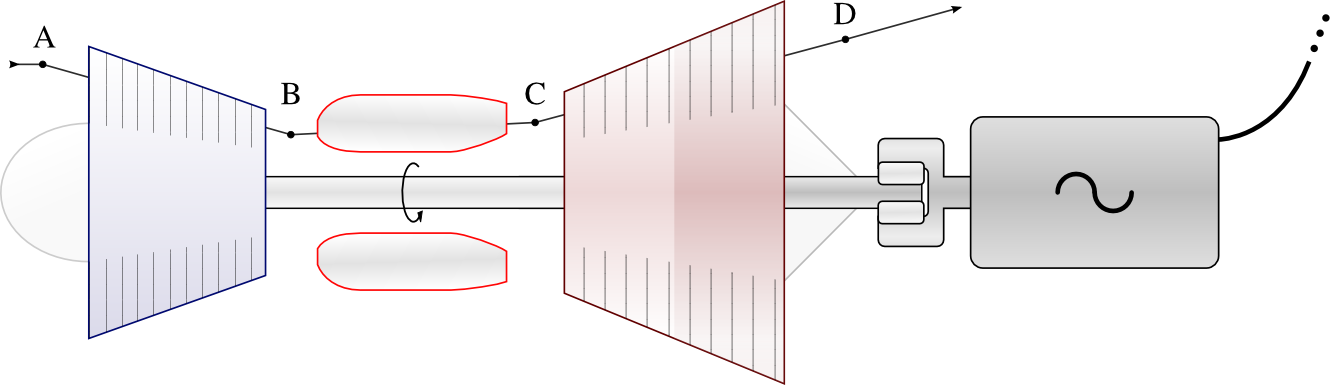
\includegraphics[width=\textwidth]{images/turbomoteur_generatrice.png}
		\end{center}
		\supercaption{Une turbomachine statique, nommée \vocab{turbomoteur}, alimentant une génératrice électrique. On tente généralement de détendre le gaz (dans la turbine, entre C et D) jusqu’à pression atmosphérique.}{schéma \ccbysa \olivier}
		\label{fig_exo_turbomoteur}
	\end{figure}
		
	\begin{itemize}
		\item L’air pénètre dans la machine à~\SI{20}{\degreeCelsius} et~\SI{1}{\bar} ; il est comprimé ($\fromatob$) jusqu’à~\SI{30}{\bar} dans le compresseur.	
		\item L’air reçoit ensuite de la chaleur par combustion, à pression constante ($\frombtoc$), jusqu’à ce que sa température atteigne \SI{1000}{\degreeCelsius}.	
		\item L’air est enfin détendu dans une turbine ($\fromctod$) jusqu’à retrouver la pression atmosphérique et être rejeté à l’extérieur.
	\end{itemize}
	
	Le compresseur est alimenté mécaniquement par la turbine et l’arbre qui les relie entraîne également la génératrice de courant.
	
	Pour étudier le rendement maximal qui pourrait être atteint par la machine, nous considérons que le compresseur et la turbine sont adiabatiques réversibles (c’est-à-dire que la compression et la détente se font de façon très lente et sans transfert de chaleur).

	\begin{enumerate}
		\item Tracez le chemin suivi par l’air pendant un cycle sur un diagramme pression-volume, de façon qualitative (c’est-à-dire sans représenter les valeurs numériques).
		\item À quelle température l’air sort-il du compresseur ?
		\item Quelle est la puissance du compresseur ?
		\item À quelle température l’air est-il rejeté dans l’atmosphère ? Quelle puissance est rejetée sous forme de chaleur dans l’atmosphère ?
		\item Quelle est l’efficacité de la machine ?
		\item Comment les quatre transferts énergétiques de cette machine théorique se comparent-ils à ceux d’une machine réelle, dans laquelle le compresseur et la turbine ne peuvent pas être réversibles ?
	\end{enumerate}


\subsubsection{Cycle d’un moteur à vapeur}
\label{exo_centrale_vapeur_cycle}

	Dans une centrale à vapeur, l’eau circule en continu en traversant quatre composants :
	
	\begin{itemize}
		\item Une pompe quasi-adiabatique dans laquelle elle rentre à l’état de liquide saturé et qui porte sa pression depuis \SI{0,5}{\bar} jusqu’à~\SI{40}{\bar} ;
		\item Une chaudière dans laquelle sa température est portée à~\SI{650}{\degreeCelsius}, à pression constante ;
		\item Une turbine quasi-adiabatique qui laisse l’eau retourner jusqu’à~\SI{0,5}{\bar} en perdant de l’énergie sous forme de travail ;
		\item Un condenseur qui refroidit l’eau à pression constante (\SI{0,5}{\bar}) jusqu’à son retour dans la pompe.
	\end{itemize}
	
	Nous acceptons les hypothèses suivantes :
		\begin{itemize}
			\item À la sortie de la turbine, la vapeur est\footnote{Après le \courshuit nous saurons prédire cette température de sortie.} à température de~\SI{110}{\degreeCelsius}.
			\item La compression dans la pompe est réversible, et la masse volumique de l’eau ne varie pas lorsqu’elle la traverse.
		\end{itemize}
	
	\begin{enumerate}
		\item Tracez le cycle suivi par l’eau sur un diagramme pression-volume et sur un diagramme température-volume, de façon qualitative.
		\item Quelle est l’efficacité du moteur ?
		\item Que se passerait-il si, pour éliminer les rejets de chaleur, on supprimait le condenseur, en connectant l’entrée de la pompe directement sur la sortie de la turbine ?
	\end{enumerate}


\subsubsection{Réfrigération industrielle}
\label{exo_refrigeration_supermache}

	Une chaîne de supermarchés fait appel à votre expertise pour évaluer la rentabilité d’un ambitieux projet de renouvellement d’une flotte de réfrigérateurs.
	
	Tous les supermarchés de l’entreprise utilisent le même modèle de réfrigérateur. Son efficacité est de~\SI{100}{\percent}.
	
	Vous vous déplacez jusqu’à un supermarché représentatif, ce qui vous permet d’effectuer des mesures et de quantifier les transferts thermiques du bâtiment. Vous mettez en évidence que :
	
	\begin{itemize}
		\item La puissance absorbée sous forme de chaleur par la chambre froide des réfrigérateurs, moyennée sur l’année, est de~\SI{80}{\kilo\watt}.
		\item L’hiver, le bâtiment perd de la chaleur avec une puissance moyenne de~\SI{400}{\kilo\watt}. Il est réchauffé avec une batterie de pompes à chaleur de \textsc{cop} \num{4}.
		\item L’été, le bâtiment absorbe de la chaleur avec une puissance moyenne de~\SI{160}{\kilo\watt}. Il est refroidi avec une batterie de climatiseurs de \textsc{cop} \num{0,9}.
		\item Pendant l’automne et le printemps, les besoins en chauffage/refroidissement sont quasi-nuls.
	\end{itemize}
	
	L’entreprise envisage de remplacer toute sa flotte de réfrigérateurs avec un modèle d’efficacité \SI{220}{\percent}, ce qui demande un investissement important. Elle compte 100 supermarchés au total, et paie l’électricité \SI{0,15}{\euroo} par \si{\kilo\watt\hour} en moyenne.
	
	Quelle serait l’économie financière annuelle générée par le changement de modèle de réfrigérateur ?


\subsubsection{Fonctionnement d’un climatiseur}
\label{exo_fonctionnement_climatiseur}

	Un climatiseur fonctionne selon le circuit schématisé en \cref{fig_exo_climatiseur}. Le fluide utilisé dans le circuit est de l’air\footnote{On utilise souvent, en pratique, des fluides qui se liquéfient et s’évaporent dans la machine ; mais le principe de fonctionnement reste le même.}\nolinebreak.
	
	\begin{figure}
		\begin{center}
		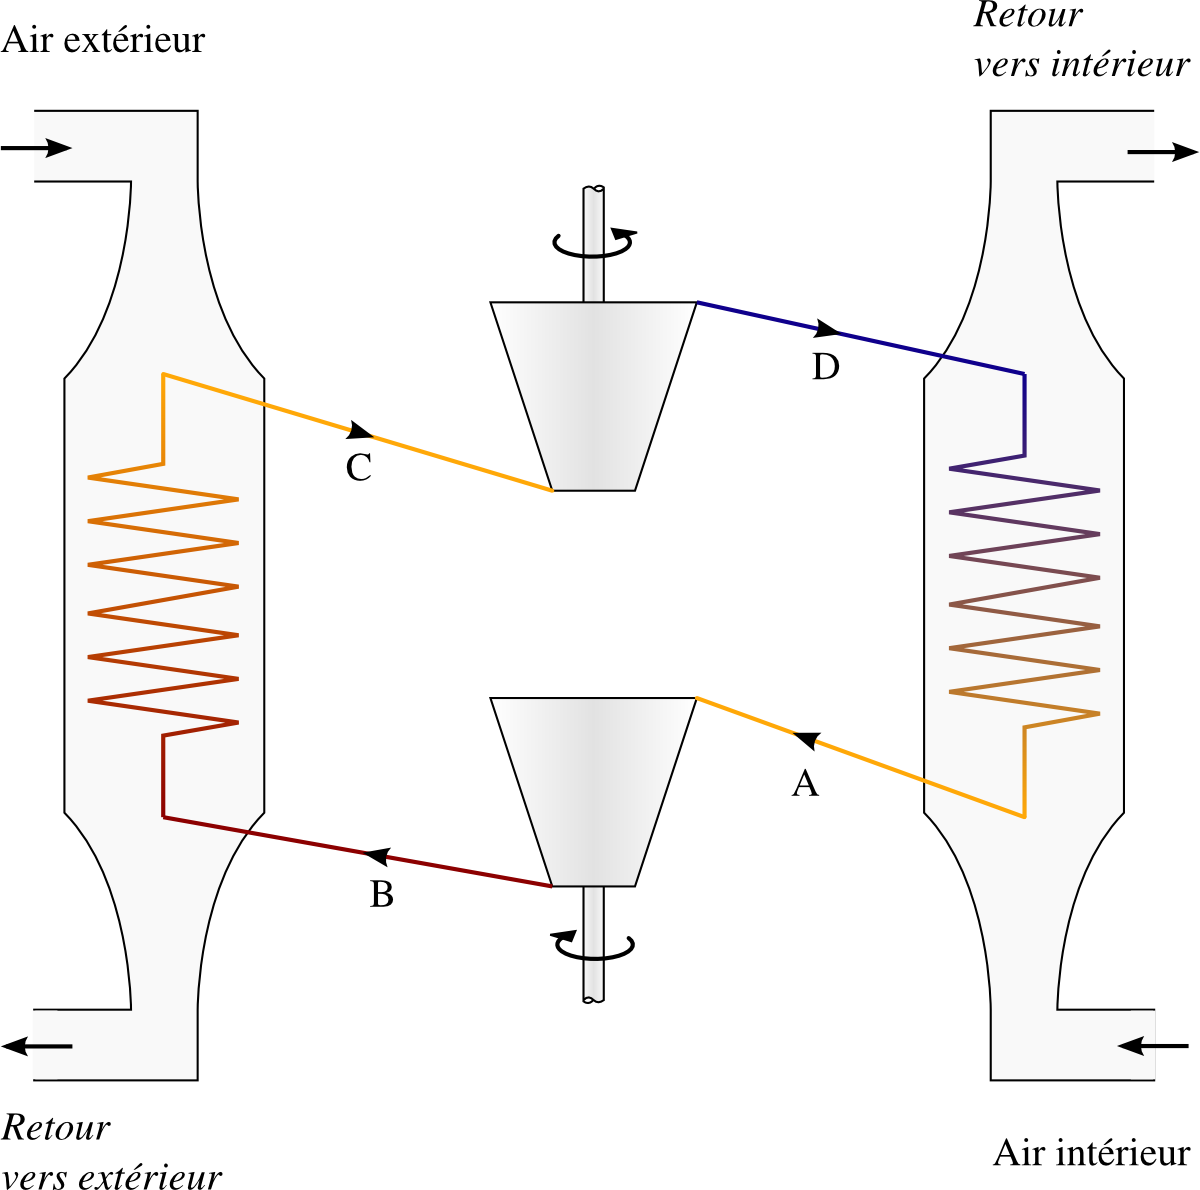
\includegraphics[width=\textwidth]{images/circuit_conditionnement_air.png}
		\end{center}
		\supercaption{Schéma de principe d’un climatiseur. L’air du circuit du climatiseur tourne en continu ($\A \to \B \to \C \to \D \to \A$), sans jamais quitter la machine.}{schéma \ccbysa \olivier}
		\label{fig_exo_climatiseur}
	\end{figure}
	
	L’air à l’intérieur du circuit y tourne de façon continue. Le compresseur et la turbine sont tous les deux adiabatiques et nous considérons qu’ils sont réversibles. Les échanges de chaleur se font à pression constante.

	Lorsqu’on met en route le climatiseur, la température extérieure et la température intérieure sont égales à~\SI{30}{\degreeCelsius}.
 
	Les températures de l’air à l’intérieur du circuit sont $T_\A = \SI{20}{\degreeCelsius}$, $T_\B = \SI{60}{\degreeCelsius}$, et~$T_\C = \SI{40}{\degreeCelsius}$.

	\begin{enumerate}
		\item Représentez l’évolution sur un diagramme pression-volume, de façon qualitative et en y représentant les transferts de travail et de chaleur.
		\item Quel est le rapport des pressions entre A et B ?
		\item Quelle est la température de l’air du circuit en D ?
		\item Calculez les puissances spécifiques pour chacun des quatre transferts énergétiques, et calculez ainsi l’efficacité du climatiseur.
		\item Le/la propriétaire souhaite obtenir un flux d’air frais à~\SI{12}{\degreeCelsius} de débit~\SI{0,25}{\metre\cubed\per\second}. Quelle puissance électrique faut-il fournir au climatiseur pour cela ?
		\item Quel sera alors le débit minimal d’air extérieur à faire circuler dans la section extérieure du climatiseur ?
		\item Pendant l’hiver, le/la propriétaire souhaite modifier le climatiseur pour le transformer en pompe à chaleur. Décrivez (de façon qualitative) une modification du circuit pour cela, et tracez l’évolution de l’air du circuit sur un nouveau diagramme pression-volume en y indiquant les transferts énergétiques.
	\end{enumerate}


\subsubsection{Pack de conditionnement}
\label{exo_pack_conditonnement}

	Un «~pack~» de conditionnement d’air est une machine thermodynamique utilisée dans les avions de transport pour pressuriser le fuselage et pour maintenir la température dans le cockpit, la cabine et les soutes à un niveau confortable quelles que soient les conditions extérieures.
	
	Les packs (souvent appelés \textsc{ecs} ou \textsc{acm}, pour \vocabe{Environment Control System} et \vocabe{Air Cycle Machine}) sont souvent placés autour du caisson de voilure dans la zone non-pressurisée des avions de ligne (\cref{fig_pack_ssj}). Une particularité intéressante de leur fonctionnement est que c’est l’air du circuit thermodynamique lui-même qui est inséré dans la cabine à destination des passagers.
	
	\begin{figure}
		\begin{center}
			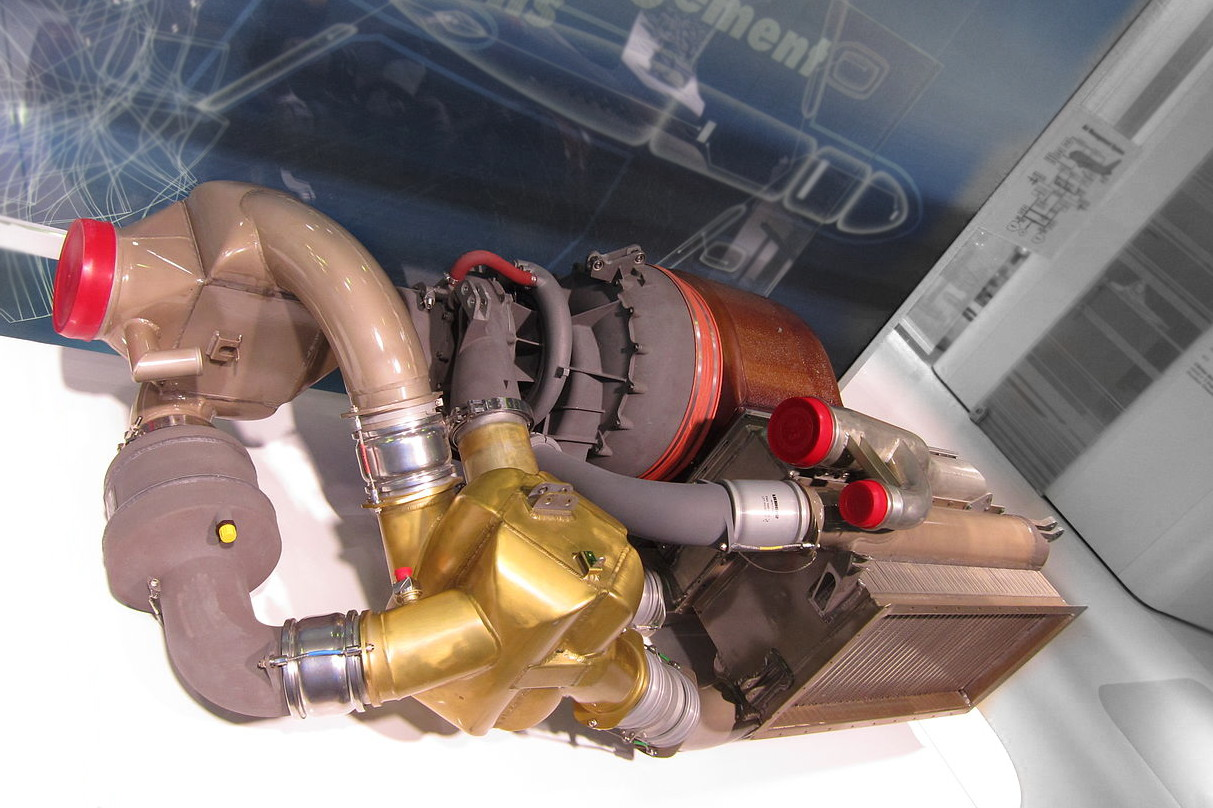
\includegraphics[height=.35\textwidth]{images/liebherr_pack.jpg}
		\end{center}
		\supercaption{Un \textsc{ecs} destiné à un \wf{Comac C919}, de longueur environ \SI{1,5}{\metre}.}{\wcfile{Air conditioning pack of Comac C919 (1).jpg}{Photo} \ccbysa \olivier}
		\label{fig_pack_c919}
	\end{figure}
	

	Nous étudions ici les fonctions de chauffage et de climatisation d’un pack : pour cela, nous simplifions la modélisation de son fonctionnement.
	
		L’air destiné à la cabine commence son chemin à l’entrée des moteurs à turbine de l’avion\footnote{Excepté lorsque l’avion, au sol, est connecté à une source d’air conditionné ou pressurisé.}. Dans le compresseur d’un de ces moteurs, sa pression est multipliée par~\num{5} pendant une évolution approximativement adiabatique réversible ; puis il est conduit jusqu’au pack.
	
		En entrant dans le pack, cet air passe par un échangeur de chaleur où il perd de la chaleur (figure~\ref{fig_pack}). Cette chaleur est prélevée par un flux d’air distinct, dit \textsc{ram} : c’est de l’air extérieur aux conditions atmosphériques, prélevé et rejeté sous le fuselage. Les circuits d’air cabine et d’air \textsc{ram} sont à des pressions très différentes et ne sont jamais mélangés.
	
	\begin{figure}
		\begin{center}
			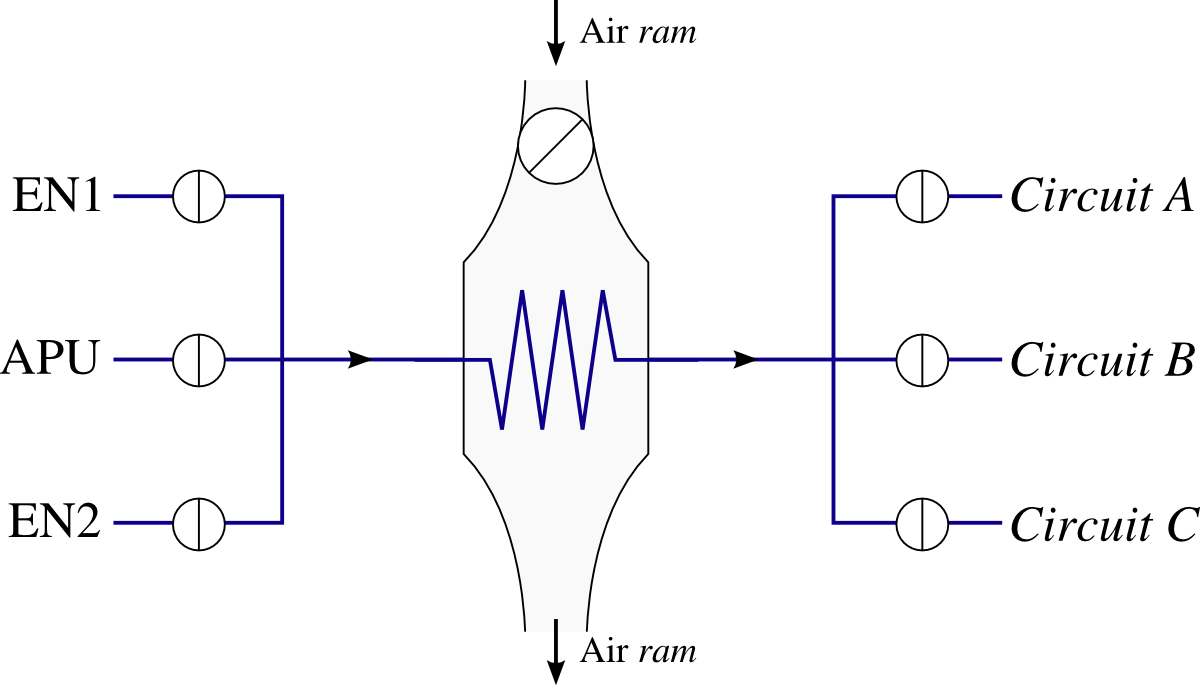
\includegraphics[width=\textwidth]{images/pack.png}
		\end{center}
		\supercaption{Circuit représentant l’air arrivant dans le pack par la gauche, en provenance des moteurs (\textsc{en1} et \textsc{en2}) ou du groupe auxiliaire de puissance (\textsc{apu}). Cet air repart dans un des trois circuits A, B ou C après avoir perdu de la chaleur au profit de l’air \textsc{ram}.}{schéma \cczero \oc}
		\label{fig_pack}
	\end{figure}

	Après son passage dans l’échangeur de chaleur, l’air du pack peut suivre trois circuits distincts avant d’arriver dans la cabine :
		\begin{description}
			\item[Le circuit A] est utilisé par temps froid, lorsque l’on souhaite porter ou maintenir la cabine à une température plus haute que la température extérieure ;
			\item[Le circuit B] est utilisé par temps modéré, lorsque la cabine doit être portée ou maintenue à température proche de la température extérieure ;
			\item [Le circuit C] est utilisé par temps chaud, lorsque les besoins en climatisation de la cabine sont importants.
		\end{description}
	
	Le pack contrôle automatiquement le débit d’air extérieur (\textsc{ram}) et sélectionne le circuit à suivre par l’air destiné à la cabine, pour porter sa température jusqu’à la valeur demandée par l’équipage au poste de pilotage (\cref{fig_320_ecs}).
	
\textbf{Circuit A : Réchauffage par temps froid}

	Dans le circuit A, l’air destiné à la cabine est simplement détendu dans une soupape (figure~\ref{fig_soupape}) avant d’être inséré dans la cabine.

	\begin{figure}
		\begin{center}
			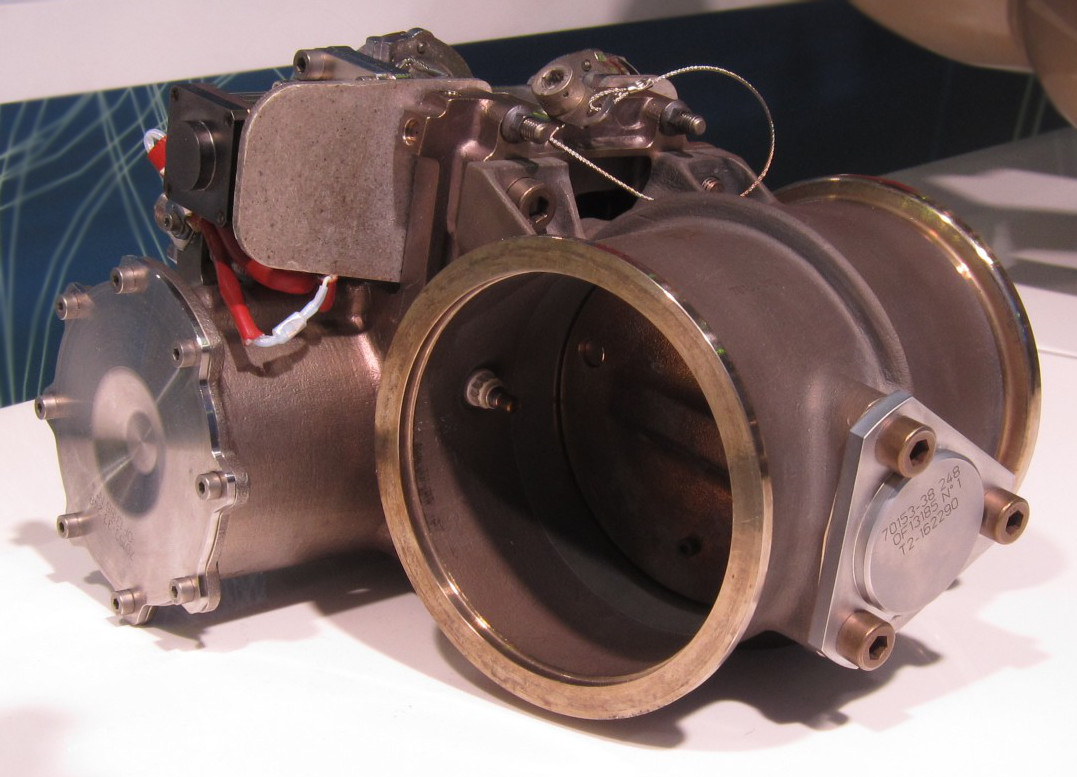
\includegraphics[height=.2\textwidth]{images/outflow_valve_1.jpg}
			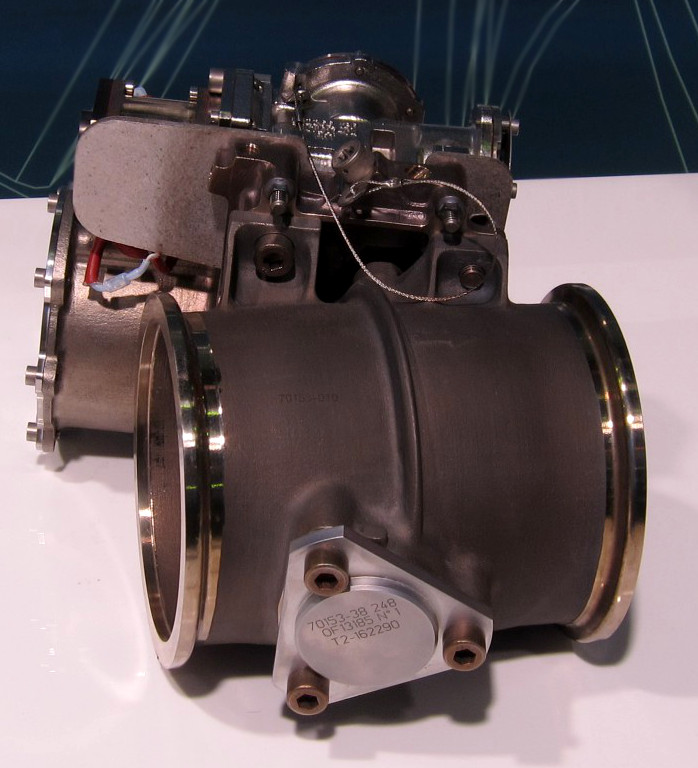
\includegraphics[height=.2\textwidth]{images/outflow_valve_2.jpg}
		\end{center}
		\supercaption{Valve de régulation de l’écoulement d’air d’un \textsc{ecs} destiné à un Comac C919.}{photos \cczero \oc}
		\label{fig_soupape}
	\end{figure}
	
	Dans la soupape, la pression chute brutalement et le volume spécifique augmente ; pourtant, aucun travail ou transfert de chaleur n’est effectué. Il s’agit d’une détente dite «~de Joule et Gay-Lussac~» (\textit{cf}. \S\ref{ch_principe_de_joule}). Le processus est entièrement irréversible.
	
	Lorsque l’avion est au sol par conditions climatiques froides (\SI{-35}{\degreeCelsius}, \SI{1}{\bar}) :
	
	\begin{enumerate}
		\item Quelle est la température \emph{maximale} de l’air que le pack peut insuffler en cabine ?\\
			(pour cela, nous fermerons entièrement le circuit d’air extérieur \textsc{ram}).
		\item Représentez l’évolution sur un diagramme pression-volume, de façon qualitative.
		\item Quel serait le débit minimal d’air extérieur à faire circuler dans le circuit \textsc{ram} pour amener \SI[per-mode=symbol]{0,5}{\kilogram\per\second} d’air conditionné à \SI{24}{\degreeCelsius} dans la cabine ?
		\item Tracez l’évolution que subirait alors l’air conditionné sur le diagramme $p-v$ plus haut.
	\end{enumerate}


	\begin{figure}
		\begin{center}
			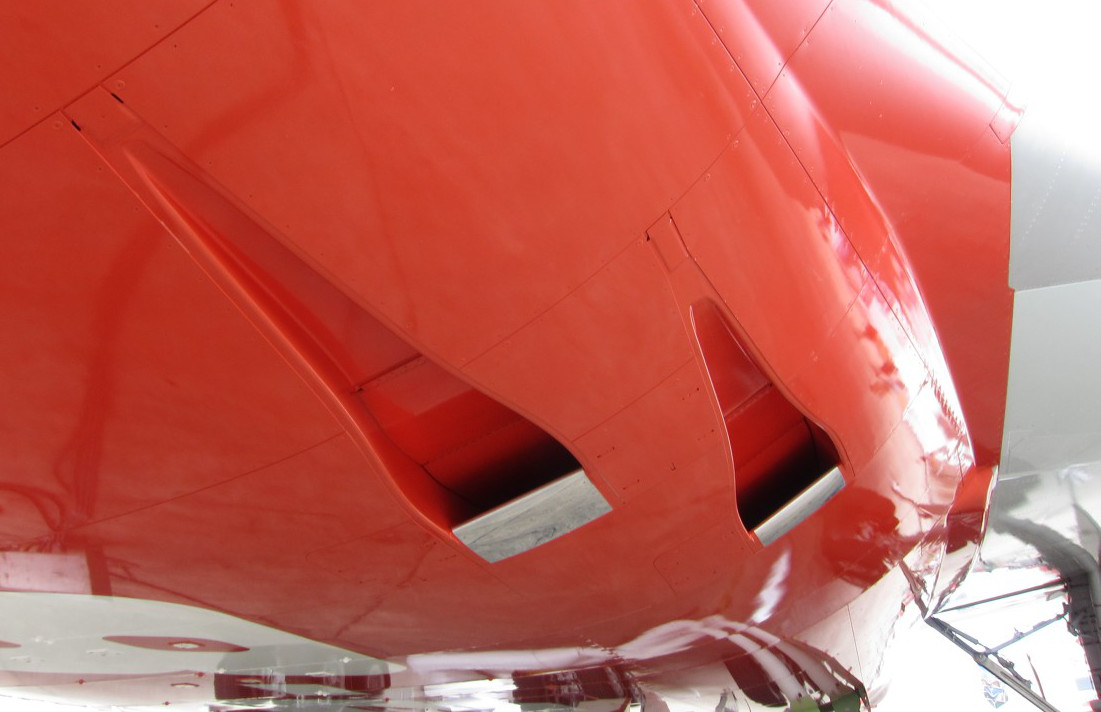
\includegraphics[height=.35\textwidth]{images/ram_pack_air_intakes_747.jpg}
		\end{center}
		\supercaption{Les entrées d’air du circuit \textsc{ram} au caisson de voilure d’un \wfd{Boeing 747-8}{Boeing 747-8I}.}{Photo \ccbysa \olivier}
		\label{fig_747_ram_intake}
	\end{figure}
	
	\begin{figure}
		\begin{center}
			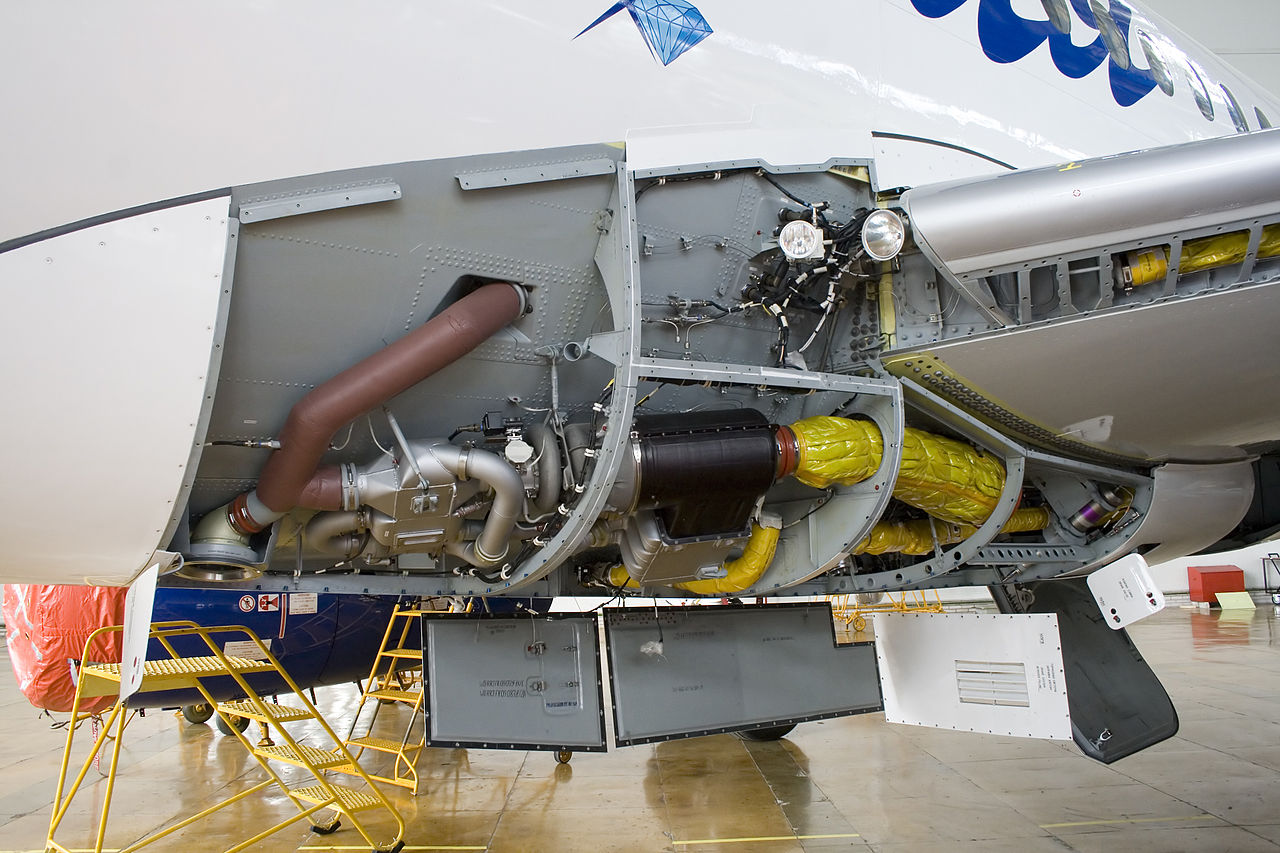
\includegraphics[width=.8\textwidth]{images/pack_sukhoi.jpg}
		\end{center}
		\supercaption{Pack de conditionnement positionné à l’emplanture d’aile d’un Sukhoi SuperJet S100}{\wcfile{Air conditioning systems of a Sukhoi Superjet.jpg}{Photo} \ccbysa A.Katranzhi}
		\label{fig_pack_ssj}
	\end{figure}


\textbf{Circuit B : Climatisation cabine par temps modéré}

	En pratique, il est possible de faire chuter la température de l’air destiné à la cabine avec un débit d’air \textsc{ram} beaucoup plus faible. Pour cette raison, lorsque les besoins en refroidissement sont importants, l’air destiné à la cabine passe par le circuit~B. Il est alors détendu à l’aide d’une turbine jusqu’à la pression cabine (\SI{1}{\bar}).  Nous considérons que la turbine est idéale (détente adiabatique réversible).
	
	Lorsque les conditions extérieures sont de~\SI{20}{\degreeCelsius}, \SI{1}{\bar} :
	
	\begin{enumerate}
	\shift{4}
		\item À quelle température l’air rentrera-t-il dans la cabine si le circuit \textsc{ram} est fermé ?
		\item Quelle énergie sera alors extraite à l’air par la turbine ?
		\item Tracez l’évolution suivie par l’air sur un diagramme pression-volume, de façon qualitative.
		\item À quelle température \emph{minimale} le circuit peut-il porter l’air destiné à la cabine ?
		\item Quelle énergie sera alors extraite à l’air par la turbine ?
		\item Tracez l’évolution sur le diagramme $p-v$ plus haut.
	\end{enumerate}

\onlyframabook{\clearpage}
\textbf{Circuit C : Climatisation cabine par temps chaud}

	Lorsque l’appareil évolue au sol par conditions climatiques très chaudes (\SI{45}{\degreeCelsius}, \SI{1}{\bar}) l’air destiné à la cabine passe par le circuit C.
	
	Au passage dans l’échangeur, sa température ne descend que jusqu’à \SI{217}{\degreeCelsius}. 
	
	Il est ensuite comprimé dans un compresseur (adiabatique réversible) jusqu’à \SI{20}{\bar}. 
	
	Il passe ensuite de nouveau par un échangeur de chaleur traversé par le circuit d’air \textsc{ram}.
	
	Enfin, il est détendu dans une turbine\footnote{En pratique, il s’agit de la turbine du circuit B.} (adiabatique réversible) jusqu’à pression atmosphérique, puis insufflé dans la cabine.
		
	\begin{enumerate}
	\shift{10}
		\item Représentez le circuit suivi par l’air au travers du pack et schématisez l’évolution sur un diagramme pression-volume.
		\item À quelle température doit-on porter l’air dans le second échangeur, avant sa détente, pour obtenir un flux d’air à \SI{5}{\degreeCelsius} dans la cabine ?
		\item Quelle est alors l’énergie sous forme mécanique que le pack reçoit ou fournit pour fonctionner ?
	\end{enumerate}

\textbf{Conclusion}
	
	\begin{enumerate}
	\shift{13}
		\item Quel est le \textsc{cop} du réchauffage généré avec le circuit A en question~3 ?
		\item Quel est le \textsc{cop} de la climatisation effectuée avec le circuit C en question~12 ?
	\end{enumerate}

	\begin{figure}[!t]
		\begin{center}
			%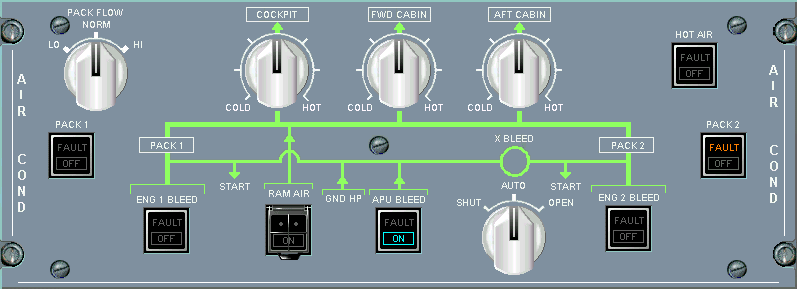
\includegraphics[width=.94\textwidth]{images/320_interface.png}
			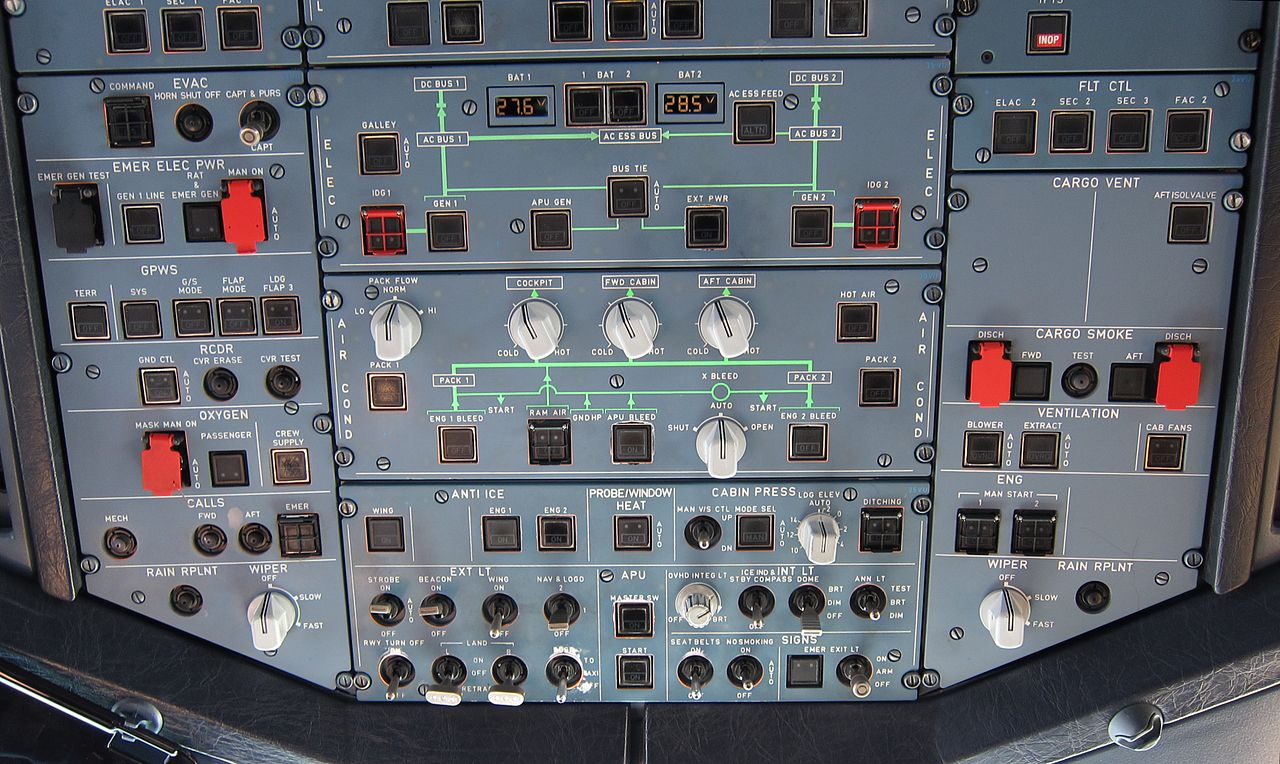
\includegraphics[width=\textwidth]{images/320_panel.jpg}
			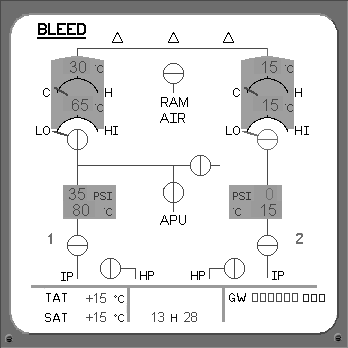
\includegraphics[width=\textwidth]{images/320_efis.png} %FIXME : vérifier le seuil d’originalité de cette image, repiquée dans un manuel de vol ou un autre…
		\end{center}
		\supercaption{Interface de contrôle de l’\textsc{ecs} au centre du panneau supérieur du cockpit d’un Airbus A320 et le panneau d’affichage \textsc{efis} correspondant.}{\wcfile{Overhead panel of an Airbus A320 during cruise.jpg}{Photo} \ccbysa \olivier}
		\label{fig_320_ecs}
	\end{figure}	

\exercisesolutionpage
\titreresultats

\begin{description}
	\item [\ref{exo_efficacite_moteur}] 
			\tab 1) $\dot Q_\inn = \frac{-\dot W_\net}{\eta_\text{moteur}} = \frac{-(\num{60e3})}{\num{0,4}} = \SI{+150}{\kilo\watt}$ ; ainsi $\dot m = \frac{\dot Q_\inn}{c_\text{carburant}} = \SI{15,4}{\kilogram\per\hour}$ (environ 12 litres par heure) ;
			\tab 2) $\dot Q_\out = -\dot Q_\inn - \dot W_\net = \SI{-90}{\kilo\watt}$.
	\item [\ref{exo_efficacite_refrigerateur}] 
			\tab $W_\net = \frac{Q_\inn}{\eta_\text{réfrigérateur}} = \SI{+83,3}{\kilo\joule}$ ; $Q_\out = -Q_\inn - W_\net = \SI{-183,3}{\kilo\joule}$.
	\item [\ref{exo_efficacite_thermopompe}] 
			\tab $\dot W_\net = \frac{-\dot Q_\out}{\eta_\text{thermopompe}} = \frac{-(\num{-4e3})}{\num{3,1}} = \SI{+1,29}{\kilo\watt}$ ; $\dot Q_\inn = -\dot W_\net - \dot Q_\out = \SI{+2,71}{\kilo\watt}$.
	\item [\ref{exo_bieres}]	
			\tab 1) Si l’on suppose que la masse volumique du liquide est égale à celle de l’eau liquide ($\rho_\text{liquide} = \SI{e3}{\kilogram\per\metre\cubed}$), la chaleur $Q_\inn$ absorbée par le réfrigérateur est $Q_\inn 
				= - Q_\text{verre} - Q_\text{liquide} - Q_\text{parois} 
				= - n_\text{bouteilles} (m_\text{verre} c_\text{verre} + m_\text{liquide} c_\text{liquide}) (\Delta T)_\text{packs} - \dot Q_\text{parois} \Delta t 
				= - \num{60} (\num{0,172} \times \num{0,75e3} + \num{0,25} \times \num{4,2e3}) \times (5 - \num{19}) - \num{10} \times 4 \times \num{3600}
				= \SI{+1134,4}{\kilo\joule}$. Ainsi, $W_\net = \frac{Q_\inn}{\eta_\text{réfrigérateur}} = \SI{+1194,1}{\kilo\joule}$.
			\tab 2) $W_\net = \SI{+1194,1}{\kilo\joule} = \SI{+1194,1}{\kilo\watt\second} = \SI{+0,332}{\kilo\watt\hour}$. Ainsi le coût revient à \SI{0,05}{\euroo} (!).
			\tab 3) La pièce sera réchauffée par le rejet $Q_\out = -Q_\inn - W_\net = \SI{-2,538}{\mega\joule}$.
			\tab 4) L’ouverture de la porte ne fait qu’augmenter la chaleur $Q_\inn$ à extraire de la chambre froide, et donc contribuera à augmenter $Q_\out$ et le réchauffement de la pièce (avec une puissance nette $\dot Q_\net = \dot Q_\inn + \dot Q_\out = -\dot W_\net$). 
	\item [\ref{exo_fonctionnement_thermopompe}]
			\tab Voir \S\ref{ch_principe_fonctionnement_réfrigérateur}, et en particulier les figures~\ref{fig_refrigerateur_climatiseur_thermopompe_so}, \ref{fig_principe_du_réfrigérateur_soupape} et \ref{fig_agencement_thermopompe}.
	\item [\ref{exo_algebre_rendement_climatiseur}]
			\tab $ \eta_\text{climatiseur} 
			\equiv \left|\frac{\dot Q_\inn}{\dot W_\net}\right| 
			= \frac{\dot Q_\inn}{\dot W_\net} 
			= \frac{\dot Q_\inn}{-\dot Q_\inn - \dot Q_\out} 
			= \frac{1}{-1 - \frac{\dot Q_\out}{\dot Q_\inn}}$.
			Or, par définition $\dot Q_\out < 0$ et $\dot Q_\inn > 0$ ; ainsi  $\frac{\dot Q_\out}{\dot Q_\inn} = -\left|\frac{\dot Q_\out}{\dot Q_\inn}\right|$.
			On~a donc $\eta_\text{climatiseur} = \frac{1}{-1 + \left|\frac{\dot Q_\out}{\dot Q_\inn}\right|}$. À vous maintenant avec les équations~\ref{eq_rendement_moteur_qin_qout} et~\ref{eq_rendement_thermopompe_qin_qout} !			
	\item [\ref{exo_refrigeration_soufflerie}] 
			\tab Les \SI{50}{\mega\watt} dépensés par la soufflante sont entièrement dissipés sous forme de frottements dans la soufflerie, et donc convertis en chaleur qu’il faut prélever si l’on veut maintenir la température constante. Ainsi $\dot W_\net = \frac{\dot Q_\inn}{\eta_\text{réfrigération}} = \SI{+62,5}{\mega\watt}$ (un sacré réfrigérateur…). Il suit que $\dot Q_\text{out} = -\dot Q_\inn - \dot W_\net = \SI{-112,5}{\mega\watt}$.
	\item [\ref{exo_generatrice_electricite_turbine}] 
			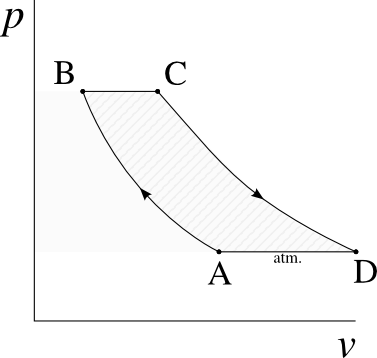
\includegraphics[height=\solutiondiagramwidth]{images/exo_sol_pv_turbomoteur_1.png}
			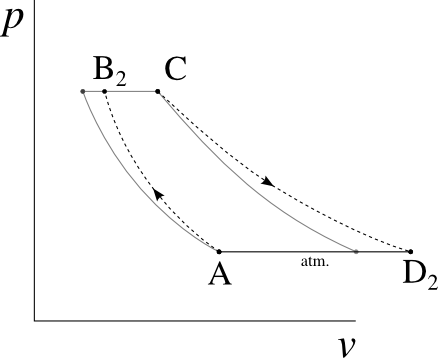
\includegraphics[height=\solutiondiagramwidth]{images/exo_sol_pv_turbomoteur_2.png}
			\tab 2) Avec l’\cref{eq_isentropique_horrible2}, $T_\B = T_\A \left(\frac{p_\B}{p_\B}\right)^{\frac{\gamma - 1}{\gamma}} = \SI{774,7}{\kelvin}$ ;
			\tab 3) Avec les équations \ref{eq_grande_sfee_deltas_h} et \ref{eq_h=cpT}, $\dot W_\fromatob = \dot m c_p (T_\B - T_\A) = \SI{+242}{\kilo\watt}$  ;
			\tab 4) Avec l’\cref{eq_isentropique_horrible2}, $T_\D = T_\C \left(\frac{p_\D}{p_\C}\right)^{\frac{\gamma - 1}{\gamma}} = T_\C \left(\frac{p_\B}{p_\A}\right)^{-\frac{\gamma - 1}{\gamma}} = \SI{481,8}{\kelvin}$. Ainsi, l’air rejeté doit perdre $\dot Q_\fromdtoa = c_p \Delta T = \SI{-94,8}{\kilo\watt}$ pour revenir à son état initial (\S\ref{ch_construction_cycle}) ;
			\tab 5) $\eta_\text{moteur} \equiv \left|\frac{\dot W_\net}{\dot Q_\inn} \right| = \left|\frac{\dot W_\fromatob + \dot W_\fromctod}{\dot Q_\frombtoc} \right| = \SI{62,3}{\percent} $ (fort honorable, mais seulement atteignable avec une turbine et un compresseur parfaits) ;
			\tab 6) Avec un compresseur réel $\dot W_{\fromatob_2} > \dot W_\fromatob$ et $T_{\B_2} > T_\B$.
						Il s’ensuit que si $T_\C$ est gardée constante, $\dot Q_{\frombtoc_2} < \dot Q_\frombtoc$.
						Néanmoins, on a encore $\dot W_{\fromctod_2} < \dot W_\fromctod$ et $T_{\D_2} > T_\D$ dans la turbine. La puissance $\dot W_\net$ diminue, le rejet $\dot Q_\out$ augmente. Nous montrerons au \courssept que le rendement diminue également.\\
					\textit{N.B. Nous avions déjà étudié ce moteur aux exercices \ref{exo_turbomoteur_puissances_spe} et surtout \ref{exo_generatrice_electrique}. Notre capacité d’analyse et de quantification des performances s’améliore à chaque fois…}		
	\item [\ref{exo_centrale_vapeur_cycle}] 
			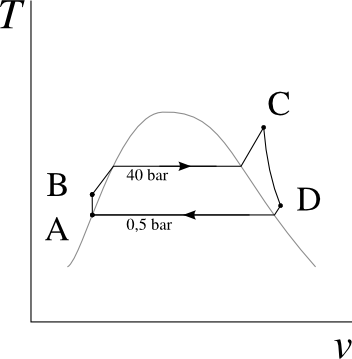
\includegraphics[height=\solutiondiagramwidth]{images/exo_sol_tv_moteur_vapeur.png}
			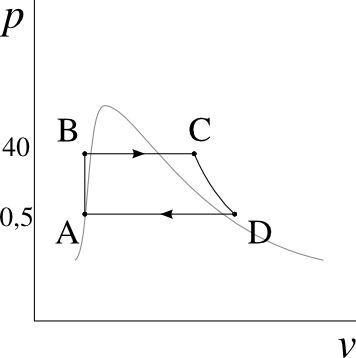
\includegraphics[height=\solutiondiagramwidth]{images/exo_sol_pv_moteur_vapeur.png}
			\tab 1) Pour s’aider à construire ces diagrammes, on peut réviser les figures~\ref{fig_t-v_eau} et~\ref{fig_p-v_eau}, ainsi que la section \S\ref{ch_lv_evolutions_elementaires}.
			\tab 2)	$h_\A = h_{L \SI{0,5}{\bar}}$ ; 
						$h_\B = h_\A + \int_\A^\B v \diff p = h_\A + v_L \Delta p $ (\ref{eq_lv_so_travail_isochore} \& \ref{eq_lv_so_chaleur_isochore} avec $q_\fromatob = 0$) ;
						$h_\C = h_{\SI{650}{\degreeCelsius} \& \SI{4}{\mega\pascal}}$ ;
						$h_\C = h_{\SI{110}{\degreeCelsius} \& \SI{0,05}{\mega\pascal}}$ ;
						Avec ces données on calcule aisément $\eta_\text{moteur} \equiv \left|\frac{w_\net}{q_\inn}\right| = -\frac{w_\net}{q_\inn} = -\frac{w_\text{turbine} + w_\text{pompe}}{q_\text{chaudière}} = -\frac{(h_\D - h_\C) + (h_\B - h_\A)}{h_\C - h_\B} = \SI{31,47}{\percent}$ (intéressant dans la mesure où on peut utiliser n’importe quel carburant).
			\tab\tab 3) Dans ce cas, la pompe ferait (presque) effectuer le chemin $\D \to \C$ à la vapeur, la ramenant à température de \SI{650}{\degreeCelsius} et rendant impossible l’apport de chaleur dans la chaudière. Nous aurions donc effectivement une machine faite d’une turbine et d’une pompe échangeant de l’eau : impossible de dégager ainsi du travail…
	\item [\ref{exo_refrigeration_supermache}] 
			\tab Dans un supermarché, au printemps comme à l’automne, l’économie d’énergie électrique permise par les nouveaux réfrigérateurs représente \SI{43,6}{\kilo\watt}.\\
			En été, la chaleur à absorber par les climatiseurs est diminuée. Il faut donc ajouter une économie de \SI{48,5}{\kilo\watt} électriques au niveau des climatiseurs.\\
			En hiver, la chaleur à apporter par les pompes à chaleur est augmentée. Il faut donc ajouter une dépense supplémentaire de \SI{10,9}{\kilo\watt} au niveau des pompes à chaleur.\\
			Au final, cela représente une économie annuelle de~\SI{1,672e12}{\joule} soit~\SI{69,7}{\kilo\euroo} par supermarché, qu’il faut comparer à l’investissement requis et aux coûts engendrés (notamment l’appel à votre expertise…).
	\item [\ref{exo_fonctionnement_climatiseur}]
				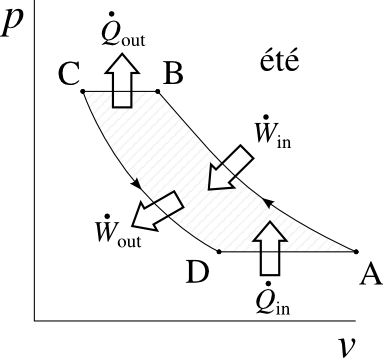
\includegraphics[height=\solutiondiagramwidth]{images/exo_sol_pv_climatiseur.png}
				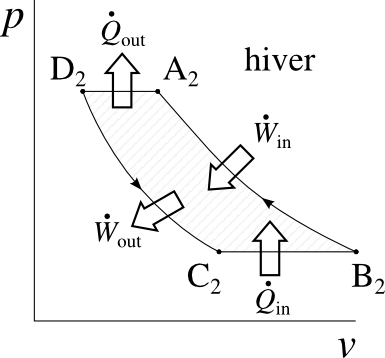
\includegraphics[height=\solutiondiagramwidth]{images/exo_sol_pv_thermopompe.png}
				\tab 2) Avec l’\cref{eq_isentropique_horrible2}, $\frac{p_\B }{p_\A} = \left(\frac{T_\B}{T_\A}\right)^{\frac{\gamma}{\gamma - 1}} = \num{1,565}$ ;
				\tab 3) Idem, détente C $\to$ D adiabatique réversible, $T_\D = T_\C \left(\frac{p_\D}{p_\C}\right)^{\frac{\gamma - 1}{\gamma}} = T_\C \left(\frac{p_\A}{p_\B}\right)^{\frac{\gamma - 1}{\gamma}} = T_\C \frac{T_\A}{T_\B} = \SI{275,6}{\kelvin}$ soit \SI{2,4}{\degreeCelsius} ;
				\tab 4) Avec les équations \ref{eq_petite_sfee_deltas_h} et \ref{eq_h=cpT}, $w_\inn = \SI{+40,2}{\kilo\joule\per\kilogram}$ ; 
						$q_\out = \SI{-20,1}{\kilo\joule\per\kilogram}$ ; 
						$w_\out = \SI{+37,76}{\kilo\joule\per\kilogram}$ ; 
						$q_\inn = \SI{+17,6}{\kilo\joule\per\kilogram}$ ; 
						Ainsi avec l’\cref{def_rendement_climatiseur_refrigerateur}, $\eta_\text{climatiseur} = \num{7,213}$
				\tab 5) On veut obtenir en 2 (bouche de sortie intérieure) $\dot m_\text{air intérieur} = \frac{\dot V_2}{v_2} = \frac{\dot V_2 p_2}{R T_2} = \SI{0,305}{\kilogram\per\second}$. 
						Il faut donc retirer à l’air intérieur une puissance $\dot Q_\text{air intérieur} = \dot m_\text{air intérieur} c_p (T_2 - T_1) = \SI{-5,51}{\kilo\watt}$ (\ref{eq_grande_sfee_deltas_h} \& \ref{eq_h=cpT}).
						Le climatiseur requerra donc $\dot W_\net = \frac{-\dot Q_\text{air intérieur}}{\eta_\text{climatiseur}} = \SI{765}{\watt}$.
				\tab 6) Pour minimiser $\dot m_\text{air extérieur}$, il faut maximiser sa température de sortie $T_4$. Or on a nécessairement $T_4 \leq T_\B$, sinon le transfert de chaleur se fait dans le mauvais sens. Ainsi $\dot m_\text{air extérieur min.} = \frac{-\dot Q_\text{out climatiseur}}{c_p (T_{4 \text{max.}} - T_3)} = -\frac{-\dot Q_\inn - \dot W_\net}{c_p (T_{4 \text{max.}} - T_3)} = \SI{0,208}{\kilogram\per\second}$ (minimum théorique).
				\tab\tab 7) En principe, il suffit d’inverser la position du compresseur et de la turbine. En pratique, il faudra également décaler les plages de températures pour permettre l’absorption de chaleur par temps froid.
	\item[\ref{exo_pack_conditonnement}]
			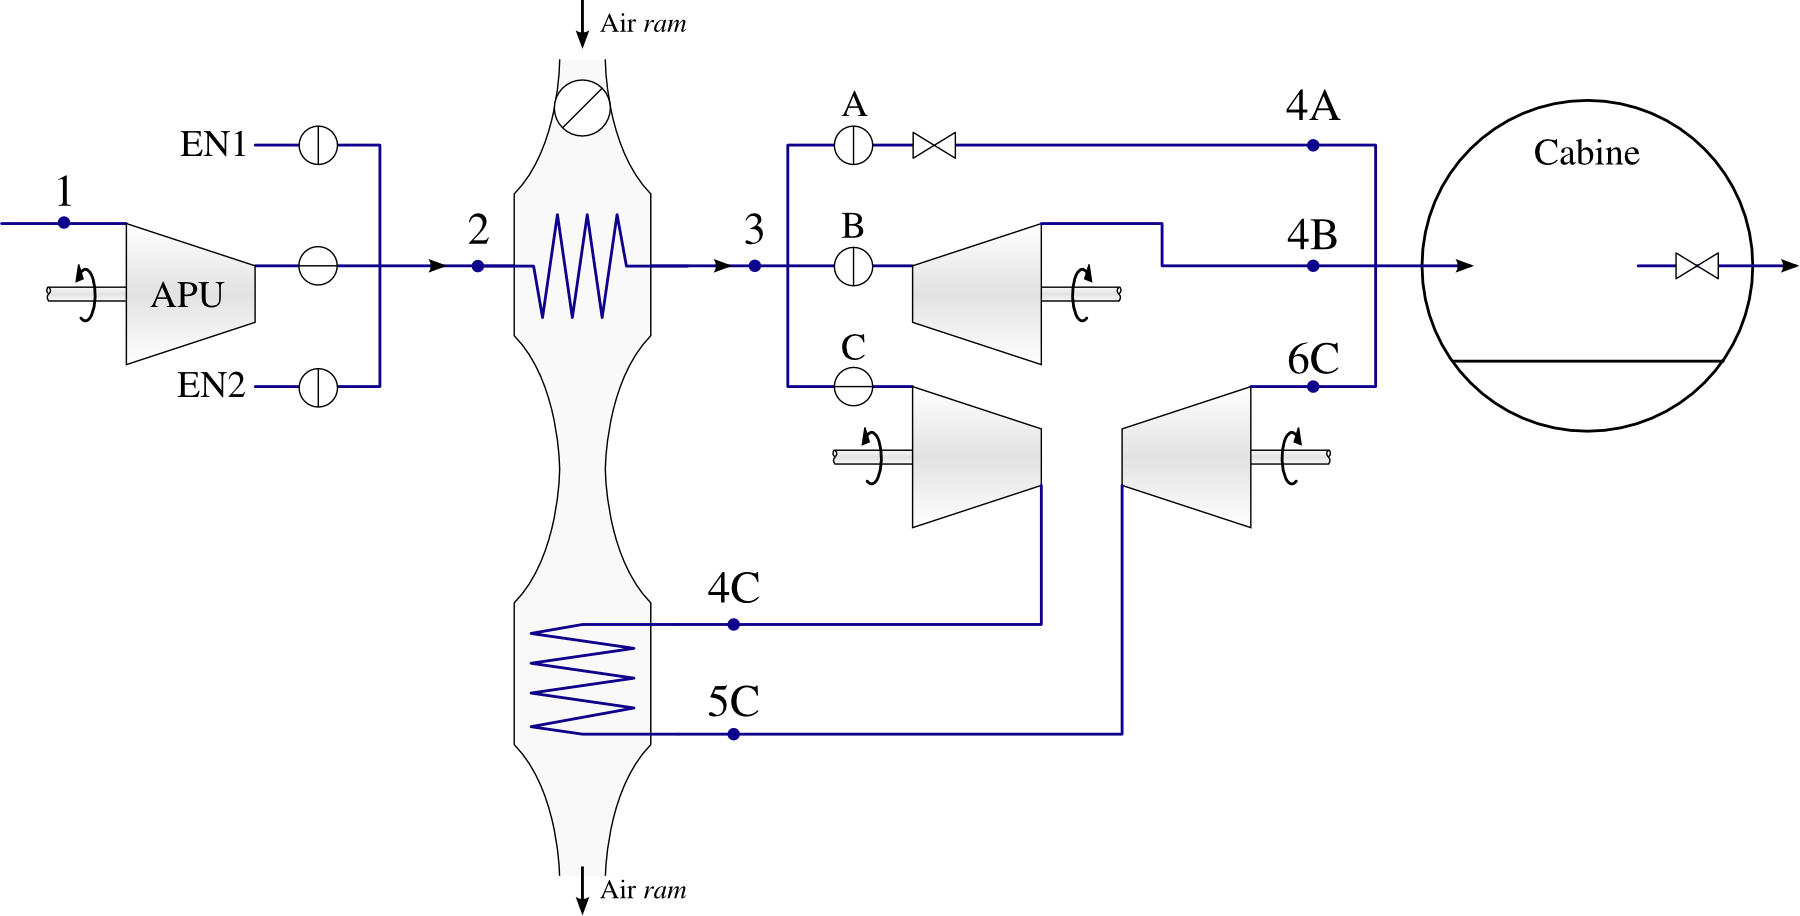
\includegraphics[width=0.9\textwidth]{images/exo_sol_circuit_acm.png}\onlyamphibook{\\}
			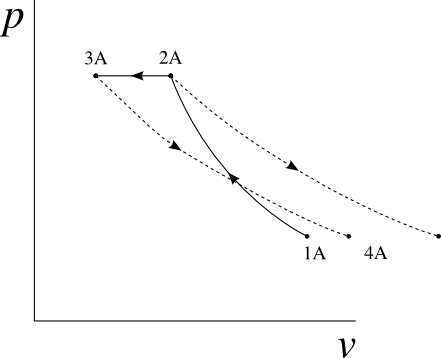
\includegraphics[height=\solutiondiagramwidth]{images/exo_sol_pv_pack_1.png}
			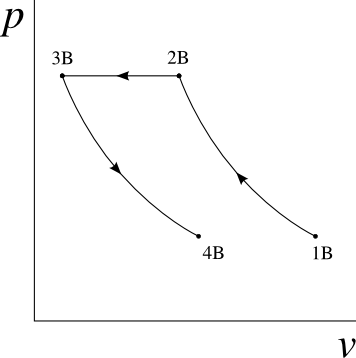
\includegraphics[height=\solutiondiagramwidth]{images/exo_sol_pv_pack_2.png}
			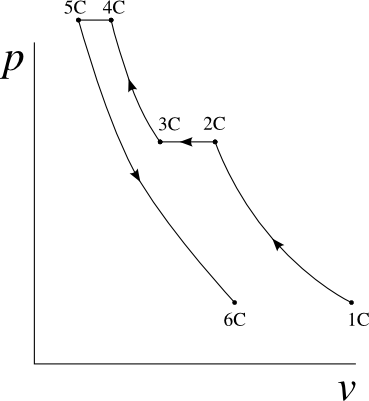
\includegraphics[width=\solutiondiagramwidth]{images/exo_sol_pv_pack_3.png}
			\tab\onlyframabook{\tab} 1) Si le circuit \textsc{ram} est fermé, alors $T_{3\A} = T_{2\A}$ ; et puisque $T_{4\A} = T_{3\A}$ (\S\ref{ch_principe_de_joule}) on obtient $T_{4\A}
			= T_{1\A} \left(\frac{p_{2\B}}{p_{1\B}}\right)^{\frac{\gamma-1}{\gamma}}
			= \SI{377,19}{\kelvin} = \SI{104,1}{\degreeCelsius}$.
			\tab 3) Dans l’échangeur \textsc{ram} on a 
				$\dot Q_\text{air cabine} = - \dot Q_\text{air \textsc{ram}}$ soit 
				$\dot m_\text{air cabine} q_\text{air cabine} =  -\dot m_\text{air \textsc{ram}} q_\text{air \textsc{ram}}$ ou encore
				$\dot m_\text{air cabine} c_p(T_{3\A} - T_{2\A}) = -\dot m_\text{air \textsc{ram}} c_p(T_\text{rejet \textsc{ram}} - T_\text{entrée \textsc{ram}})$. Ainsi, $m_\text{air \textsc{ram}}$ est minimal lorsque $T_\text{rejet \textsc{ram}}$ est maximal, or on a nécessairement $T_\text{rejet \textsc{ram}} \leq T_{2\C}$. Ainsi, 
				$\dot m_\text{air \textsc{ram} min.} = -\dot m_\text{air cabine} \frac{T_{3\A} - T_{2\A}}{T_{2\C} - T_\text{entrée \textsc{ram}}} = \SI{0,29}{\kilogram\per\second}$ (soit environ \SI{200}{\liter\per\second} à l’entrée).				
			\tab 5) Si le circuit \textsc{ram} est fermé, alors $T_{3\B} = T_{2\B}$ ; on a $T_{4\B} 
			= T_{3\B} \left(\frac{p_{4\B}}{p_{3\B}}\right)^{\frac{\gamma-1}{\gamma}}
			= T_{2\B} \left(\frac{p_{1\B}}{p_{2\B}}\right)^{\frac{\gamma-1}{\gamma}}
			= T_{1\B} = \SI{293,15}{\kelvin} = \SI{20}{\degreeCelsius}$.
			\tab 6) $w_\text{turbine B} = c_p (T_{4\B} - T_{3\B}) = -w_\text{compression B} = \SI{-172}{\kilo\joule\per\kilogram}$
			\tab 8) On obtient $T_{4\B min.}$ lorsque $T_{3\B} = T_{3\B min.} = T_\text{extérieur}$. Alors $T_{4\B min.} = T_{3\B min.} \left(\frac{p_{4\B}}{p_{3\B}}\right)^{\frac{\gamma-1}{\gamma}} = \SI{185,1}{\kelvin} = \SI{-88,1}{\degreeCelsius}$ (résultat purement hypothétique bien sûr).
			\tab 9) Elle diminue : $w_\text{turbine B2} = c_p (T_{4\B min.} - T_{3\B min.}) = \SI{-108,6}{\kilo\joule\per\kilogram}$.
			\tab 12) $T_{5\C} = T_{6\C} \left(\frac{p_{5\B}}{p_{6\B}}\right)^{\frac{\gamma-1}{\gamma}} = \SI{654,6}{\kelvin} = \SI{381,5}{\degreeCelsius}$. 
			\tab 13) On calcule d’abord $T_{4\C} = T_{3\C} \left(\frac{p_{4\C}}{p_{3\C}}\right)^{\frac{\gamma-1}{\gamma}} = \SI{728,4}{\kelvin}$. Dans le pack les transferts de travail sont de $w_\text{pack} 
			= w_\text{compresseur pack} + w_\text{turbine pack}
			= c_p(T_{4\C} - T_{3\C}) + c_p(T_{6\C} - T_{5\C})
			= \SI{-138,9}{\kilo\joule\per\kilogram}$ ;
			Ainsi l’air dépense un travail net dans le pack, qui reçoit en permanence de l’énergie sous forme pneumatique (mécanique).
			\tab 14) Pour calculer ces \textsc{cop}, il faut compléter les cycles en faisant retourner l’air aux conditions d’entrée depuis la cabine (\S\ref{ch_construction_cycle}). 
			En question~3 on a $\eta_\text{thermopompe} 
			= \left|\frac{q_\out}{w_\inn}\right| 
			= -\frac{c_p (T_{4\A} - T_{1\A})}{c_p (T_{2\A}-T_{1\A})} 
			= \num{0,424}$ (rare application où un \textsc{cop} inférieur à \SI{100}{\percent} est acceptable).
			\tab 15) En question~12 on a $\eta_\text{climatiseur} = \left|\frac{q_\inn}{w_\inn}\right| = \frac{c_p(T_{1\C} - T_{6\C})}{c_p (T_{2\C} - T_{1\C} + T_{4\C} - T_{3\C} + T_{6\C} - T_{5\C})} = \num{0,842} $.\\
			En pratique toutefois, le travail net développé par l’air dans le pack n’est pas récupéré : il est rejeté par frottement dans l’air \textsc{ram}. On a donc $w_\net = c_p(T_{2\C} - T_{1\C})$ et le \textsc{cop} est diminué.
			\tab Quelques commentaires de fin : 1) En réalité les évolutions adiabatiques ne sont pas réversibles, ce qui réduit plus encore les rendements calculés ici. 2) Les faibles valeurs de ces rendements découlent des compromis effectués pour réduire l’encombrement, la complexité et surtout le poids des systèmes embarqués. Dans cette application, la puissance mécanique disponible est élevée, l’énergie pneumatique est largement disponible, et les dépassements en volume et en poids ont des conséquences démesurées. 3) Dans les appareils les plus récents (dits \textit{plus électriques}) tels le \wfd{Boeing 787}{B787} et l’\wfd{Airbus A350 XWB}{A350}, les packs sont désormais alimentés à l’électricité, et non plus au moyen de l’air-même destiné à la cabine.
\end{description}
